\chapter{Vision}
	Im Rahmen der Semesterarbeit "`A Practical JavaScript-Only Video-Over-IP Communication Plattform"' wird eine
	Video-Over-IP-Applikation entwickelt, die vollständig im Browser läuft.
	
	Die Applikation läuft in modernen Browser ohne Plugins oder die Installation lokaler Software.
			
	\begin{figure}[H]
		\centering
		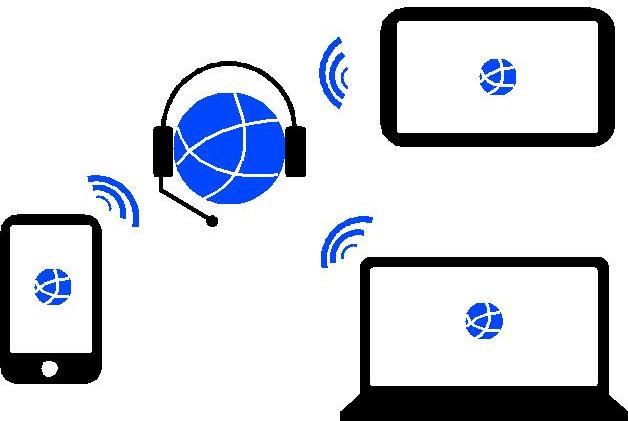
\includegraphics[width=0.5\textwidth]{../projektdokumentation/img/plattformUnabhaengigkeit.jpg}
		\label{plattformUnabhaengigkeit}
	\end{figure}
	
	Durch den offenen Standard "`WebRTC"' ist die Applikation auf jedem modernen
	Gerät benutzbar, welches den Standard umsetzt und genug Leistung für Audio- und
	Videokommunikation bereitstellt.
	
	Durch die einfache Benutzung ist die Applikation auch für technisch nicht
	versierte Benutzer zugänglich.
	
	Das integrierte Kontaktmanagement kann mit verschiedenen Importformaten umgehen und einfach um weitere Quellen erweitert werden. Dazu gibt es eine Adressbuchschnittstelle.
	
	Die Applikation kann um beliebige Signalingchannel erweitert werden. Somit ist
	es unter anderem möglich, die Applikation um Signaling über SIP oder XMPP zu
	erweitern. Dazu gibt es eine Channelschnittstelle.
	
	
	\section{Ziele}
		Im Projekt sollen die folgenden konkreten Ziele erreicht werden:
		\begin{itemize}
			\item Audio- und Videokommunikation zwischen zwei Teilnehmern.
			\item Signaling\footnote{Benachrichtigen eines anderen Peers über eine Verbindungsanfrage und Austausch von Verbindungsparametern} über beliebige Channels, Referenzimplementation eines Channels mit XHR.
			\item Adressbuchimport von beliebigen Quellen, Referenzimplementationen für
			JSON- und vCard-Import sowie eines Online-Adressbuches über eine JSON-Schnittstelle.
			\item Speichern von Adressbüchern und Benutzerinformationen im Browser (Local Storage\cite{MDN-LocalStorage}).
			\item Verschlüsselte Kommunikation zwischen den Clients. Die Kommunikation
			der Signaling-Channel-Referenzimplementation muss nicht zwingend
			verschlüsselt werden, da diese automatisch verschlüsselt wird, sobald die
			Verbindung mit TLS geschützt ist.
			\item Unterbricht die Verbindung, so soll der Stream automatisch weiterlaufen, sobald die Verbindung wieder verfügbar ist.
		\end{itemize}
		
	\section{Abgrenzung}
		\begin{itemize}
			\item Kommunikation mit mehreren Teilnehmern ist nicht Teil der Arbeit, es
			soll jedoch sichergestellt werden, dass dies später umgesetzt werden könnte.
			\item Für Adressbuchimport und Signaling-Channel sollen nur API und je eine
			Referenzimplementation umgesetzt werden und keine Implementationen für diverse Formate.
		\end{itemize}
		
		
	\section{Optionale Erweiterungen}
		Optional könnte die Applikation um einige praktische Funktionen erweitert werden:		
		\begin{itemize}
			\item Chat
			\item Austausch von Dateien
			\item Konferenzschaltung
			\item Screensharing, soweit die Browser solche Funktionalität überhaupt schon
			unterstützen
		\end{itemize}
		
		
	\section{Mehrwert gegenüber bestehenden VoIP-Lösungen}
		\subsection{Mehrwert gegenüber proprietären Diensten wie Skype, Google
		Hangout, FaceTime}
			\begin{description}
				\item[Komplette P2P-Verschlüsselung] Sowohl Videokommunikation wie
				Chatnachrichten laufen verschlüsselt komplett P2P. Der
				Signaling-Channel-Anbieter hat keinen Zugriff auf die Schlüssel.
				Entsprechend kann die Kommunikation nicht abgehört werden und auch
				serverseitig keine Backdoor eingebaut werden.
				\item[Plattformunabhängig] Skype, Google Hangout und FaceTime sind nur auf
				Geräten verfügbar, für die die Entwicklerunternehmen eine App anbieten.
				Unsere App ist auf jeder Plattform verfügbar, die einen genug modernen Browser bietet.
				\item[Erweiterbarkeit] Skype, Google Hangout und FaceTime lassen sich nicht
				um Adressbuchtypen oder Signaling-Mechanismen erweitern.
				\item[Anbieterunabhängigkeit] Skype und FaceTime lassen Kommunikation mit
				fremden Diensten nicht zu. Durch die Erweiterbarkeit unserer Applikation ist
				dies gewährleistet.
			\end{description}
		\subsection{Mehrwert gegenüber bestehenden WebRTC-Diensten wie SIPML5}
			\begin{description}
				\item[Serverdienste]
				SIPML5\footnote{\hyperlink{http://sipml5.org/}{http://sipml5.org/}} bietet
				auch Support für nicht-WebRTC-fähige Geräte und nicht-WebSocket-fähige
				SIP-Server. Ensprechend ist für SIPML5 eine Serverkomponente notwendig, die
				einen SIP-Proxy beinhaltet und die MediaStreams konvertiert. Unsere
				Applikation bietet zwar weniger Gerätesupport, benötigt dafür jedoch keine
				Serverkomponente. Mit der Verbreitung von WebRTC-fähigen Browsern und WebSocket fähigen SIP Servern würde eine entsprechende Server-orientierte Architektur sowieso obsolet.
				\item[Updatezyklen] WebRTC wird nur von den neusten Browsern unterstützt.
				Entsprechend sind die Nutzer angehalten, einen modernen Browser zu verwenden
				oder ihren alten zu aktualisieren. Durch die wegfallende Unterstützung für
				ältere Browser und nur teilweise implementierte Schnittstellen fällt unsere
				Applikation wesentlich schlanker aus.
				\item[Sicherheit] Die Videokommunikation unserer Applikation läuft in jedem
				Fall P2P. Der Benutzer kann sicher sein, dass sein Datenstrom nicht über einen Server läuft, auf dem er entschlüsselt und mitgeschnitten wird.
			\end{description}
		\subsection{Mehrwert gegenüber klassischen SIP Applikationen}
			Klassische SIP-Applikationen ermöglichen zwar eine plattformunabhängige und
			providerunabhängige Nutzung, bieten jedoch immer noch den Nachteil, dass
			eine Softwareinstallation notwendig ist.
			Unsere Applikation kann auch auf Clients genutzt werden, deren Benutzer keine Rechte zur Softwareinstallation besitzen.
			
			
	\section{Motivation}
		Motivation zur Entwicklung der Applikation sind vor allem die fehlenden
		offenen und unabhängigen Alternativen zu proprietären Diensten wie Skype,
		Google Hangout oder FaceTime und die Notwendigkeit für SIP-Services eine
		Applikation zu installieren.
		